\documentclass{article}
\author{}

\usepackage{graphicx}
\usepackage{wrapfig}
\usepackage{enumerate}
\usepackage{hyperref}
\usepackage{float}
\usepackage[margin = 2.25cm]{geometry}
\usepackage[table]{xcolor}
\usepackage{fancyhdr}
\hypersetup{
  colorlinks = true,
  urlcolor = blue
}
\setlength\parindent{0pt}
\pagestyle{fancy}
\fancyhf{}
\rhead{College of Engineering, Construction and Living Sciences\\Bachelor of Information Technology}
\lfoot{Practical 10 Django 4: Template Inheritance, Static Files \& CDNs \\Version 2, 2021}
\rfoot{\thepage}


\begin{document}

\begin{figure}
	\centering
	
\includegraphics[width=50mm]{./img/logo.png}
\end{figure}

\title{College of Engineering, Construction and Living Sciences\\Bachelor of Information Technology\\IN608: Intermediate Application Development Concepts\\Level 6, Credits 15\\\textbf{Practical 10 Django 4: Template Inheritance, Static Files \& CDNs}} 
\date{}
\maketitle

\textbf{Due Date:} 07-05-2021 at 5pm \\ 

In this practical, you will complete a series of tasks covering today's lecture. This practical is worth 2\% of the final mark for the IN608: Intermediate Application Development Concepts course. \\

Before you start, in your practicals repository, create a new branch called \textbf{10-practical}.

\section*{Task} 
Create a Django project called \texttt{dog}. \texttt{cd} to \texttt{dog}, create a virtual environment \& install Django. Create an app called \texttt{practical10cdns}. Please ensure you configure your app in \texttt{dog/settings.py} \& \texttt{dog/urls.py}. In the \texttt{practical10cdns} directory, copy \& paste \texttt{practical09dogsearch/models.py}, \texttt{practical09dogsearch/views.py}, \texttt{practical09dogsearch/urls.py} \& \texttt{templates/practical09dogsearch} from the last practical. Please ensure you change all \texttt{practical09dogsearch} references to \texttt{practical10cdns}. In \texttt{practical10cdns}, create a directory called \texttt{static} \& a sub-directory called  \texttt{practical10cdns}. \texttt{static/practical10cdns} directory is where all your static files, i.e., \texttt{CSS}, \texttt{JavaScript}, images, etc are stored. \\

In \texttt{practical10cdns/models.py}, add a new field called \texttt{image}. \texttt{image} is an \texttt{ImageField} type. Please ensure you apply migrations by running the appropriate commands. In \texttt{fixtures}, update \texttt{dogs.json} to include an \texttt{image} key with an \texttt{image} value, i.e., \texttt{afghan-hound.jpg}. Images of dogs have been provided to you in the \texttt{10-django-4-template-inheritance-static-files-cdns/img} directory. Copy \& paste the \texttt{img} directory into \texttt{static/practical10cdns}. In order to use the \texttt{ImageField}, the \texttt{Pillow} Python module must be installed. Run the command \texttt{pipenv install Pillow} to install the \texttt{Pillow} Python module. Also, \texttt{MEDIA\_URL = '/img/'} must be declared in \texttt{settings.py}. This is the URL used for managing stored files, i.e., images. \\

In \texttt{templates/practical10cdns}, create an HTML file called \texttt{base.html}. This is the file which \texttt{index.html} \& \texttt{results.html} will extend from. Include the \texttt{BootstrapCDN} \texttt{link} tag \& three \texttt{script} tags. Style your \texttt{index.html} \& \texttt{results.html} as you wish using \texttt{Bootstrap}. \\

Run the command \texttt{python manage.py runserver} then navigate to \href{http://127.0.0.1:8000/practical10cdns/}{http://127.0.0.1:8000/practical10cdns/} 

\begin{figure}[H]
  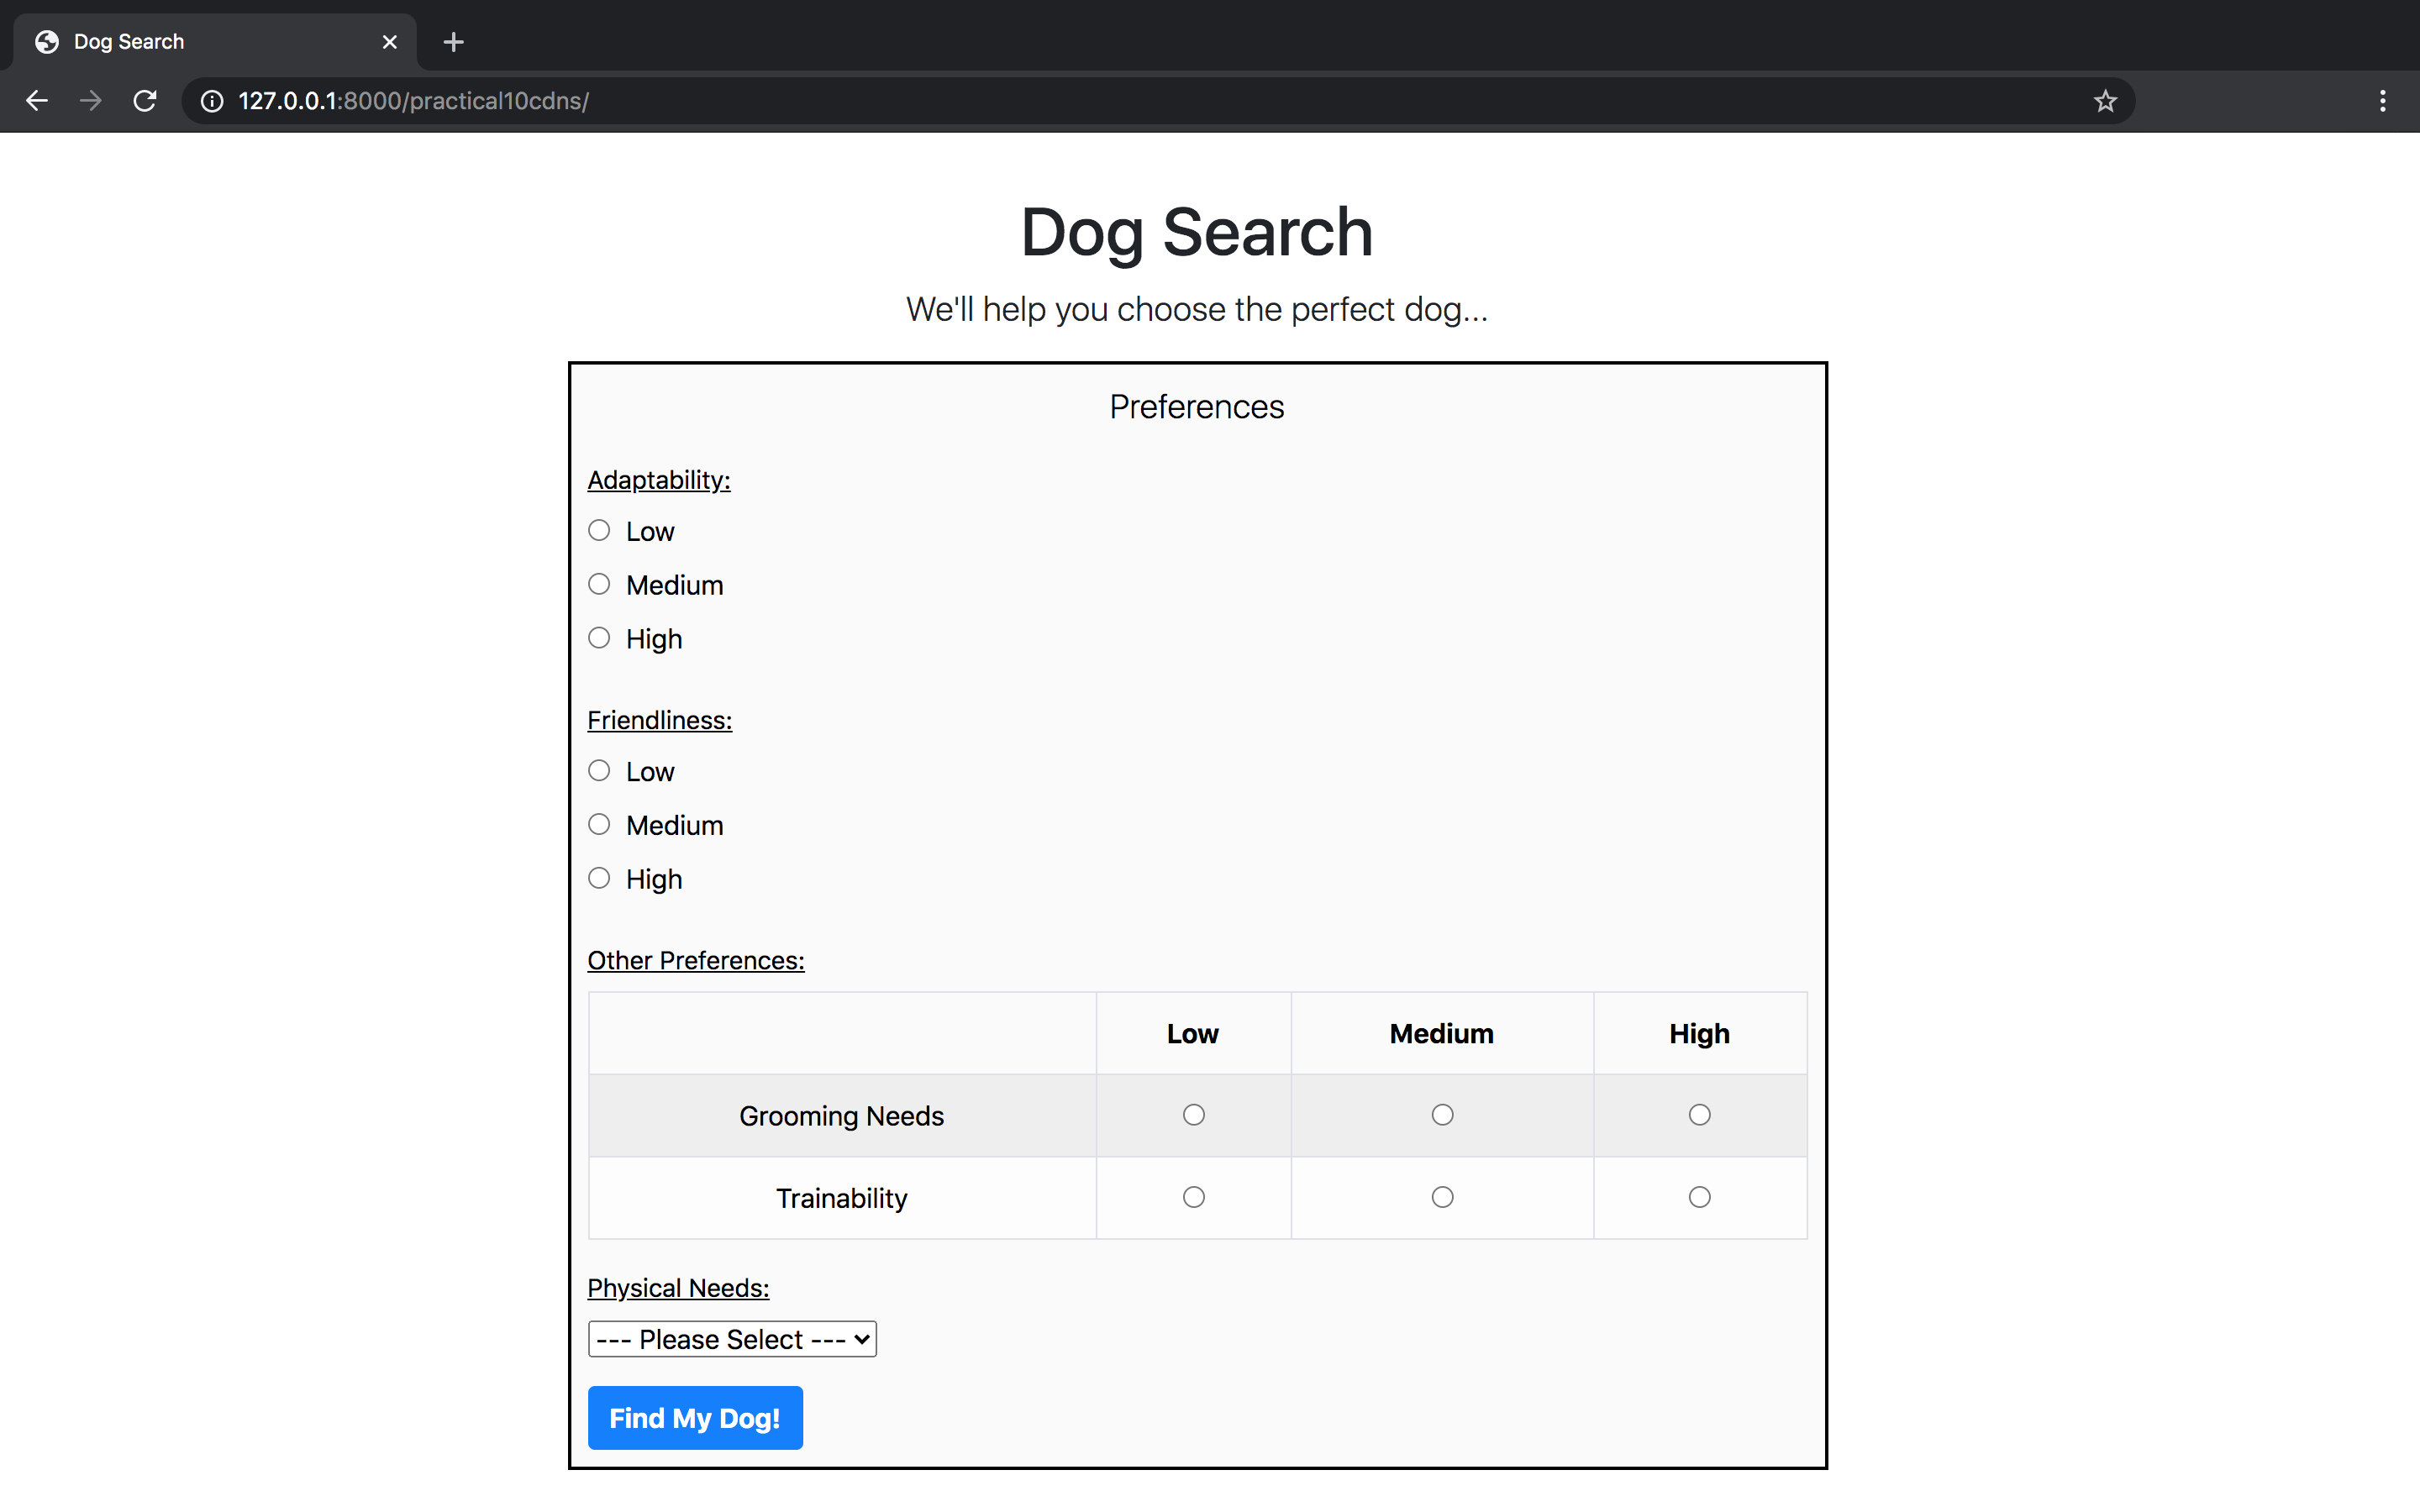
\includegraphics[width=175mm, height=100mm]{./img/10-expected-dog-search-1.png}
  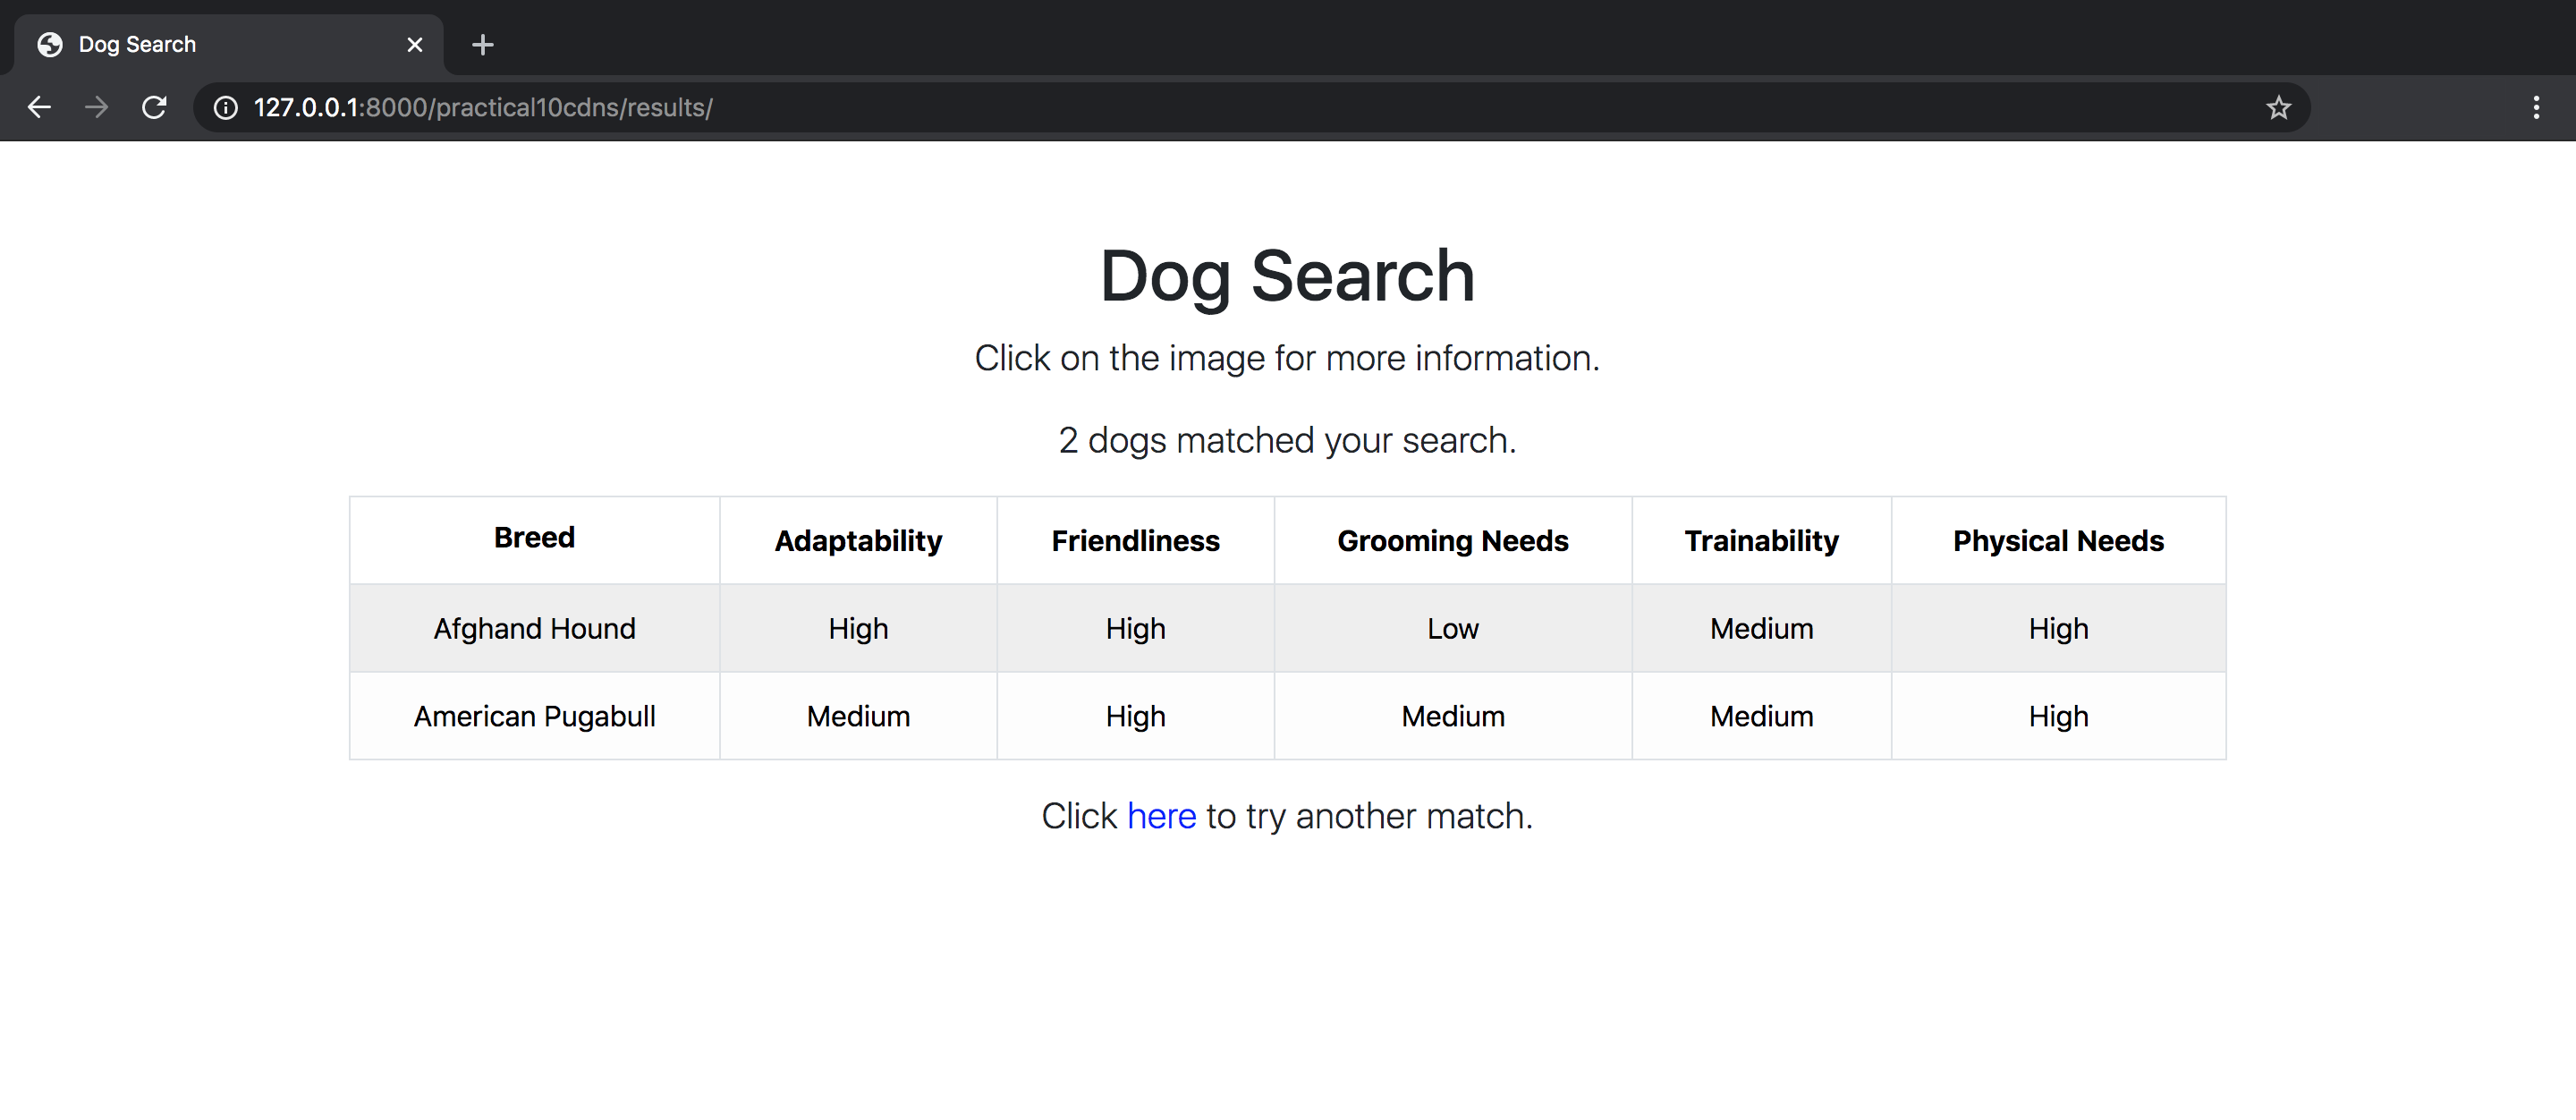
\includegraphics[width=175mm, height=75mm]{./img/10-expected-dog-search-2.png}   
\end{figure}

\begin{figure}[H]
  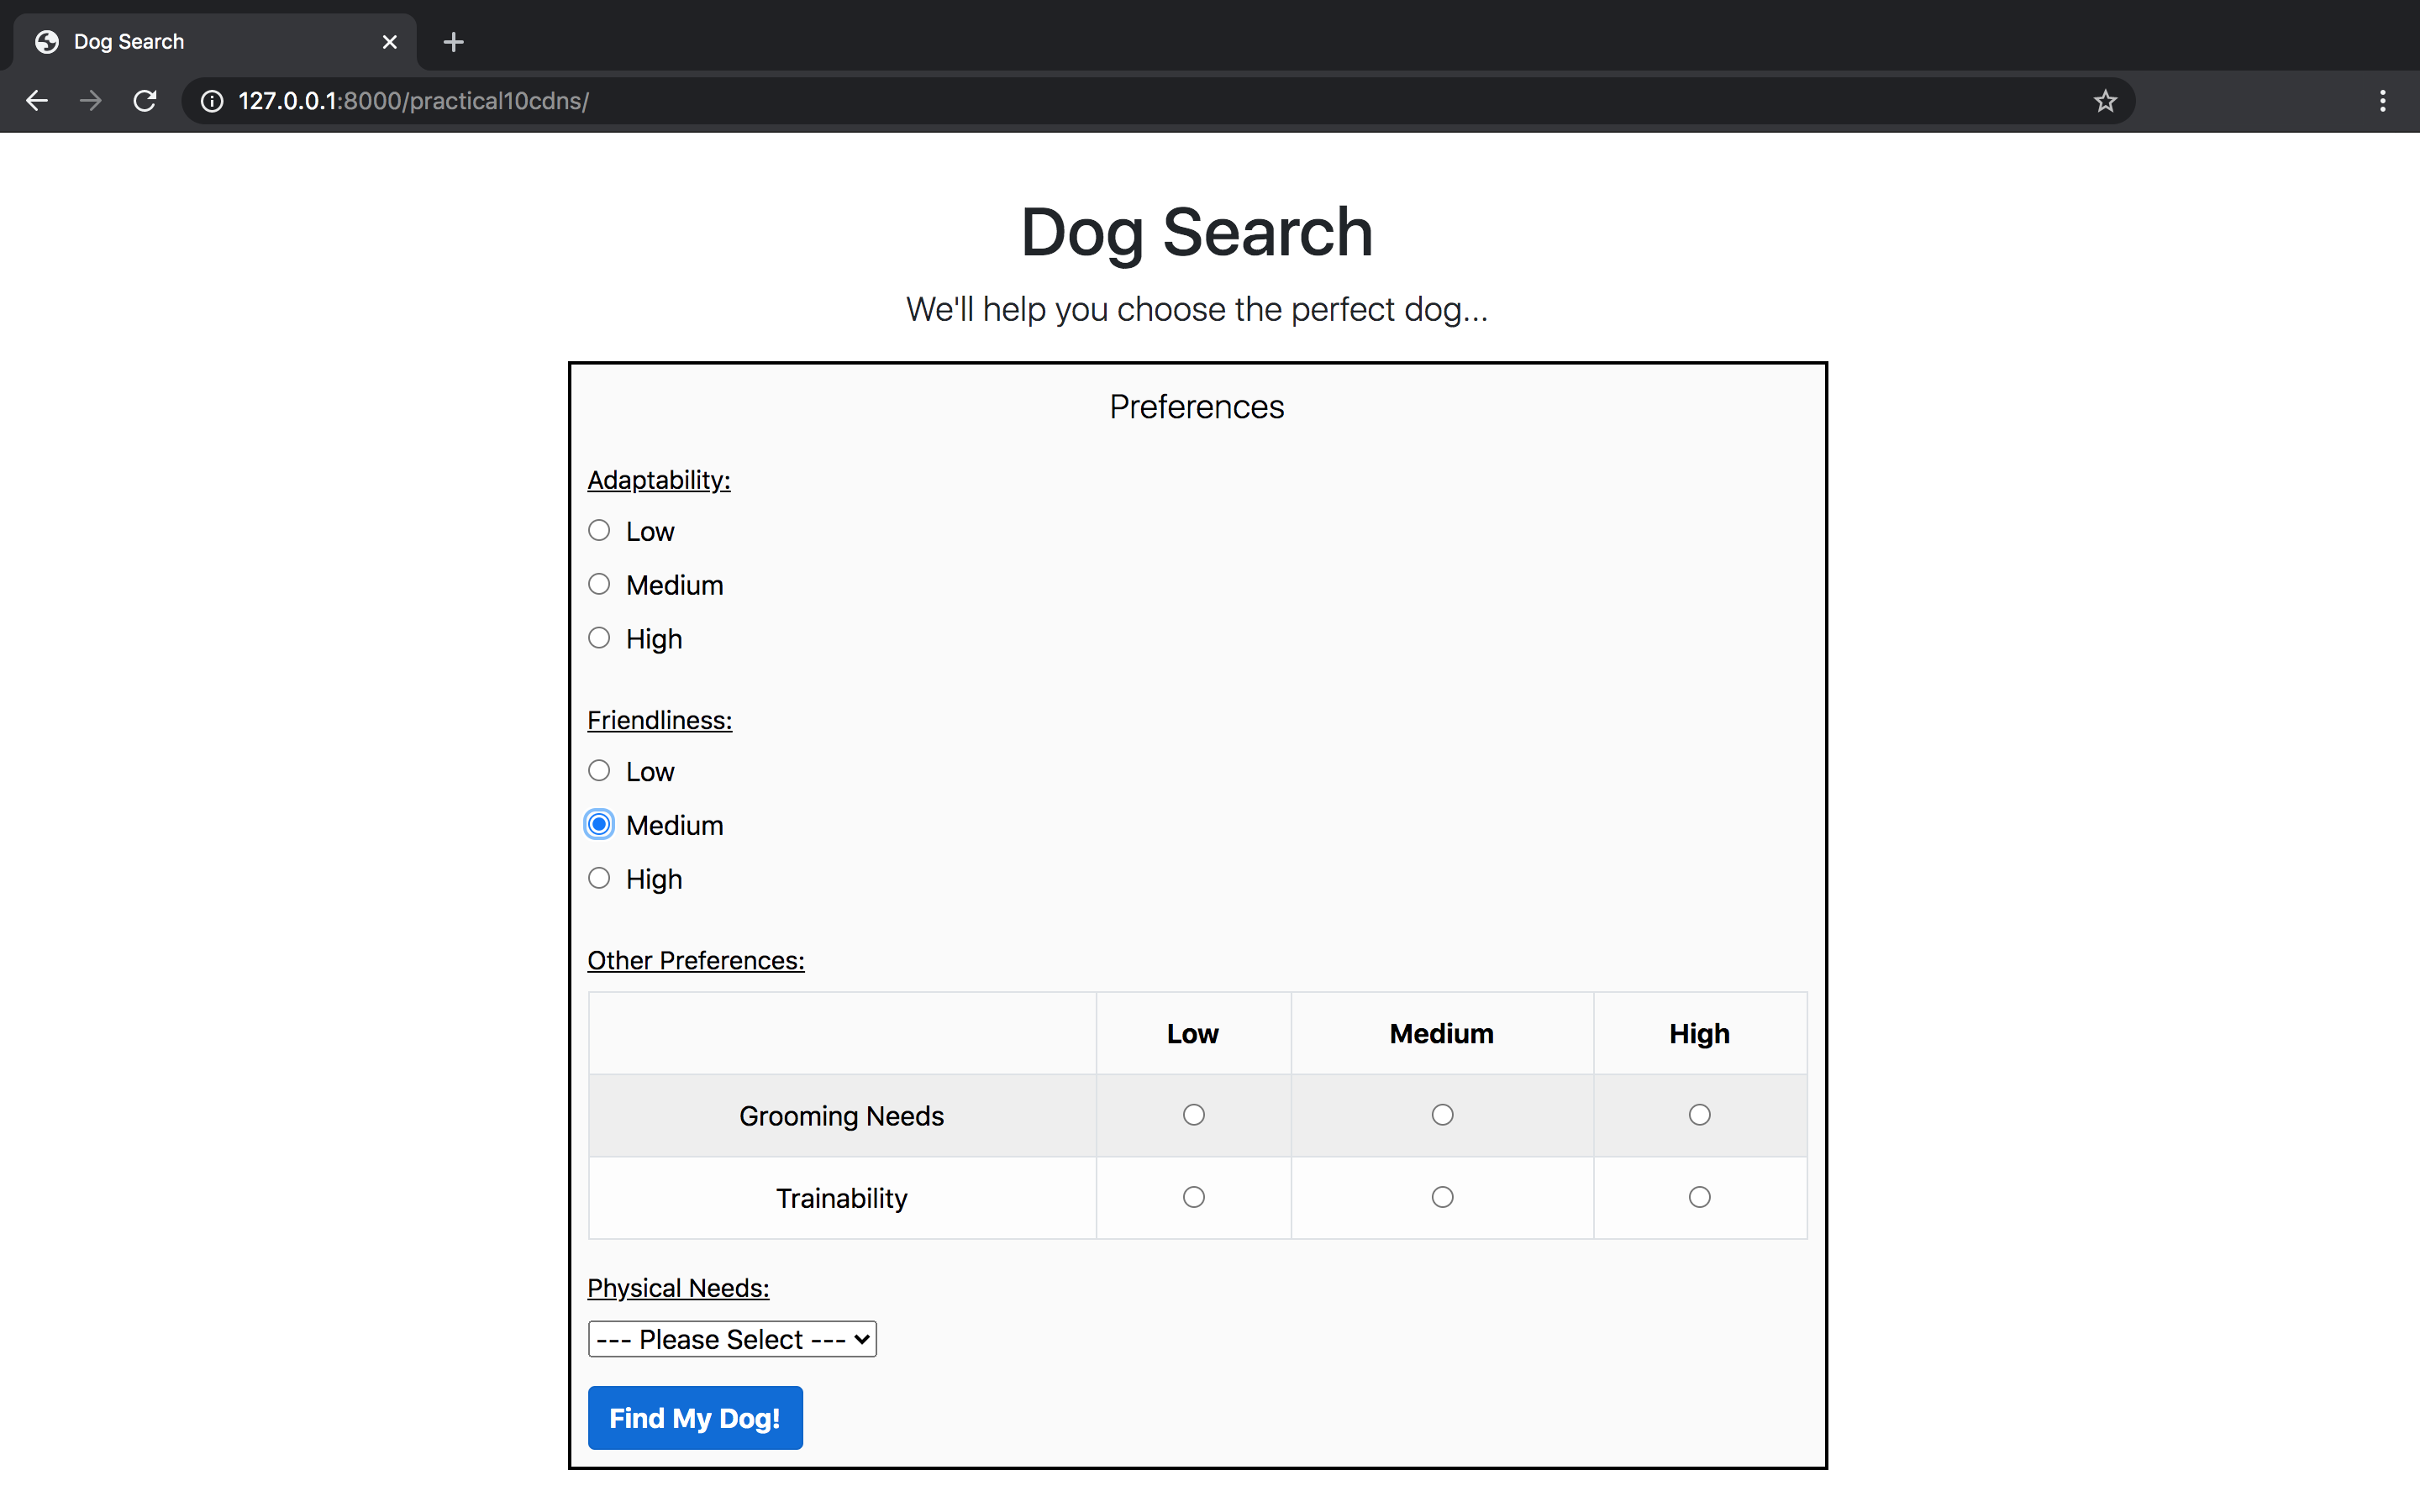
\includegraphics[width=175mm, height=100mm]{./img/10-expected-dog-search-3.png}
  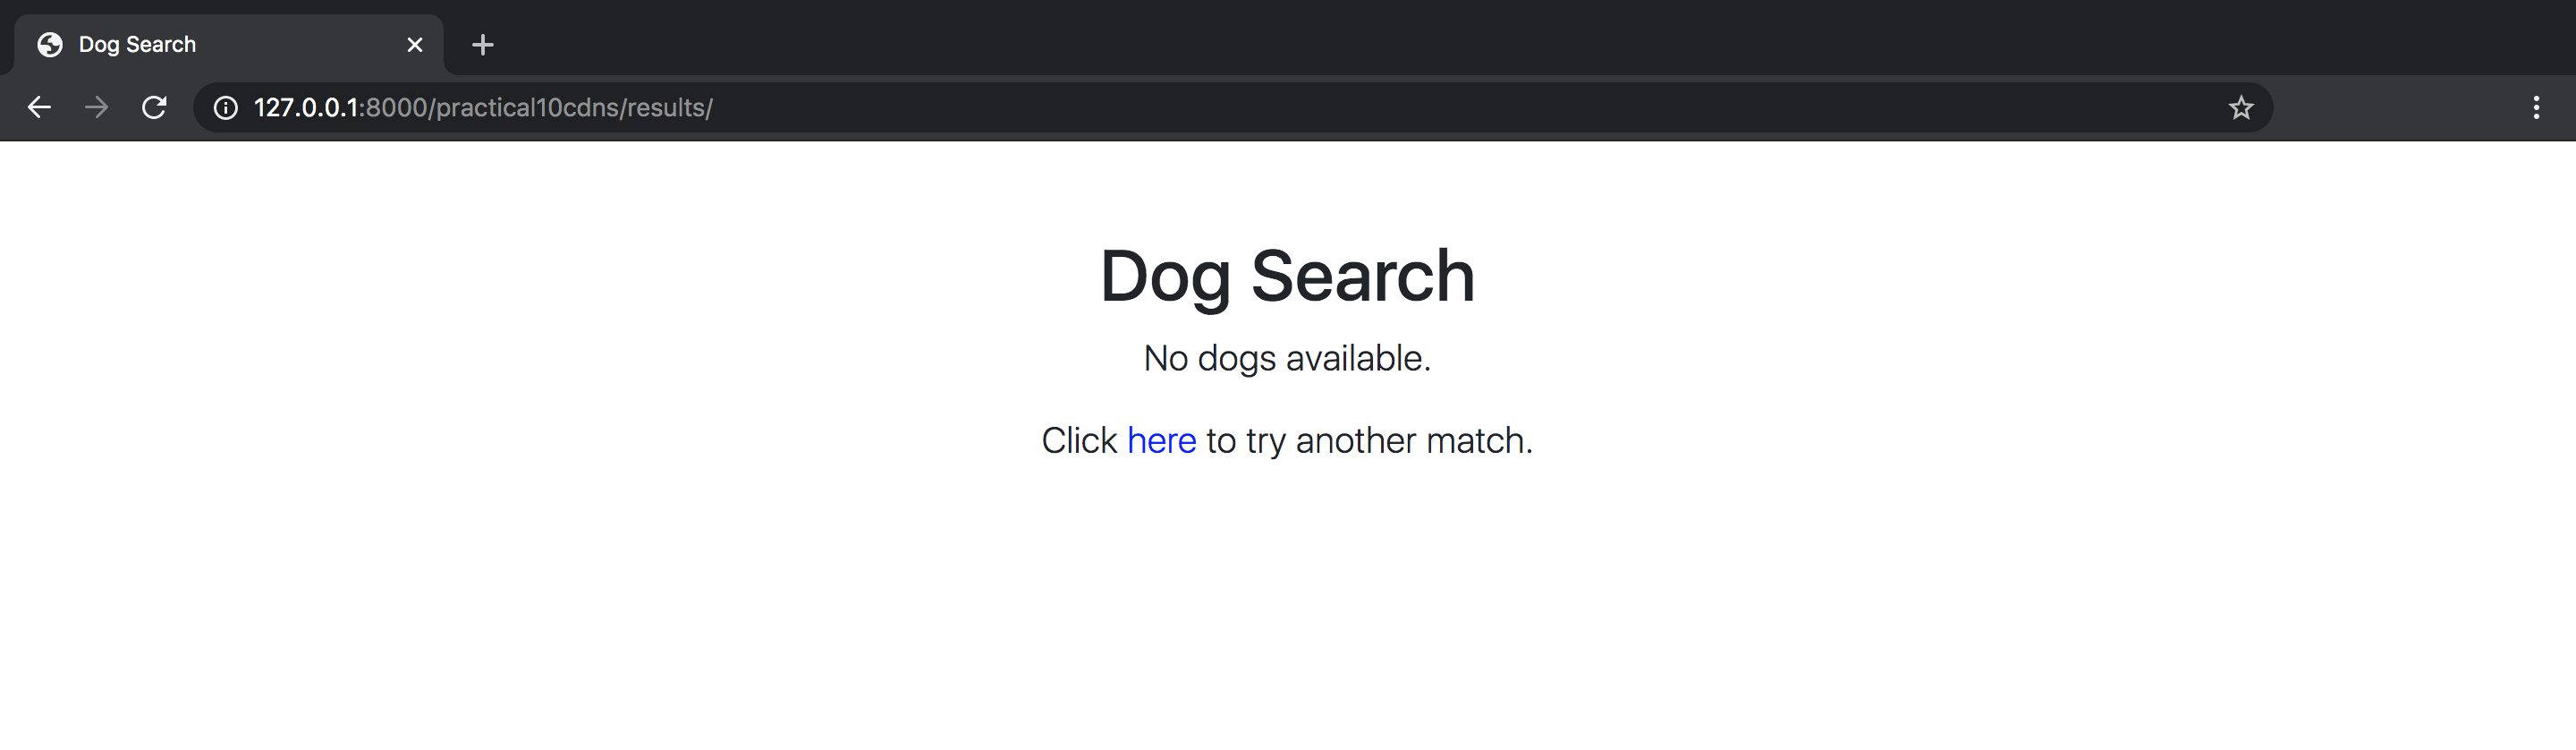
\includegraphics[width=175mm, height=55mm]{./img/10-expected-dog-search-4.png}
\end{figure}

In \texttt{results.html}, for each \texttt{Dog} object in the \texttt{QuerySet}, add a \texttt{button input} to row of \texttt{Dog} data. When a \texttt{button input} is clicked, a modal should display the \texttt{Dog} object's \texttt{image}, \texttt{height}, \texttt{weight} \& \texttt{life\_span}. 

\begin{figure}[H]
  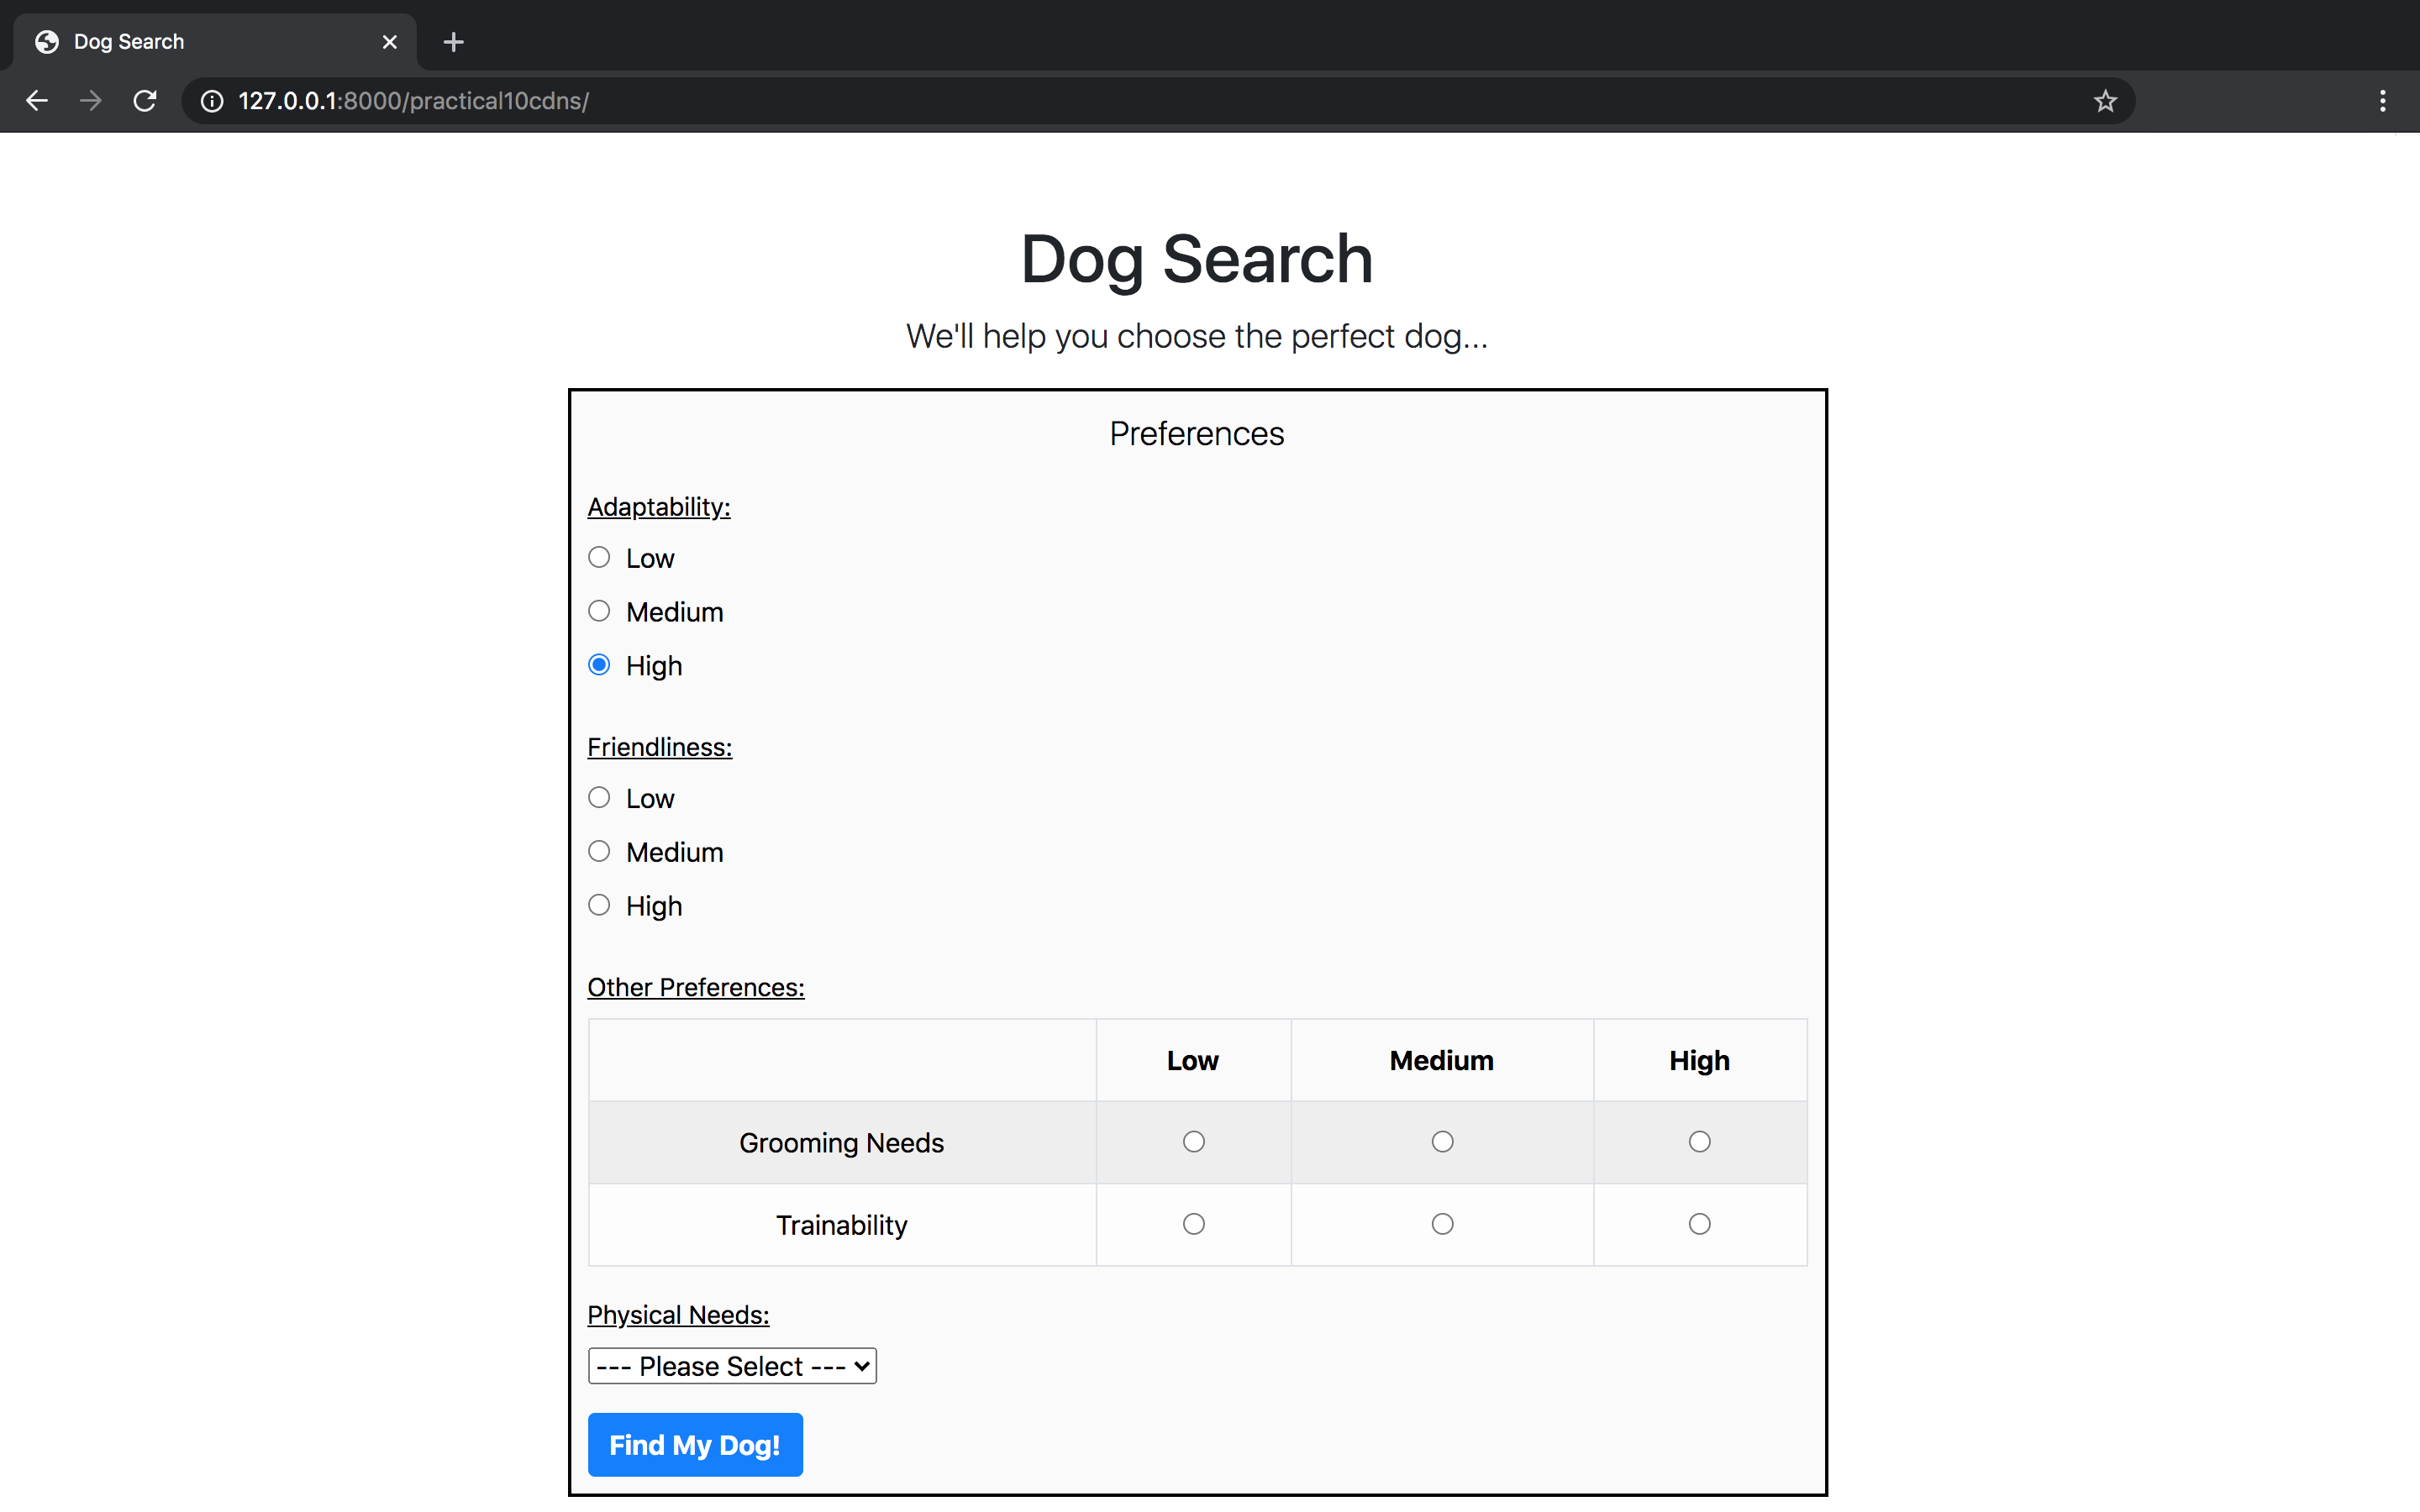
\includegraphics[width=175mm, height=100mm]{./img/10-expected-dog-search-5.png}
  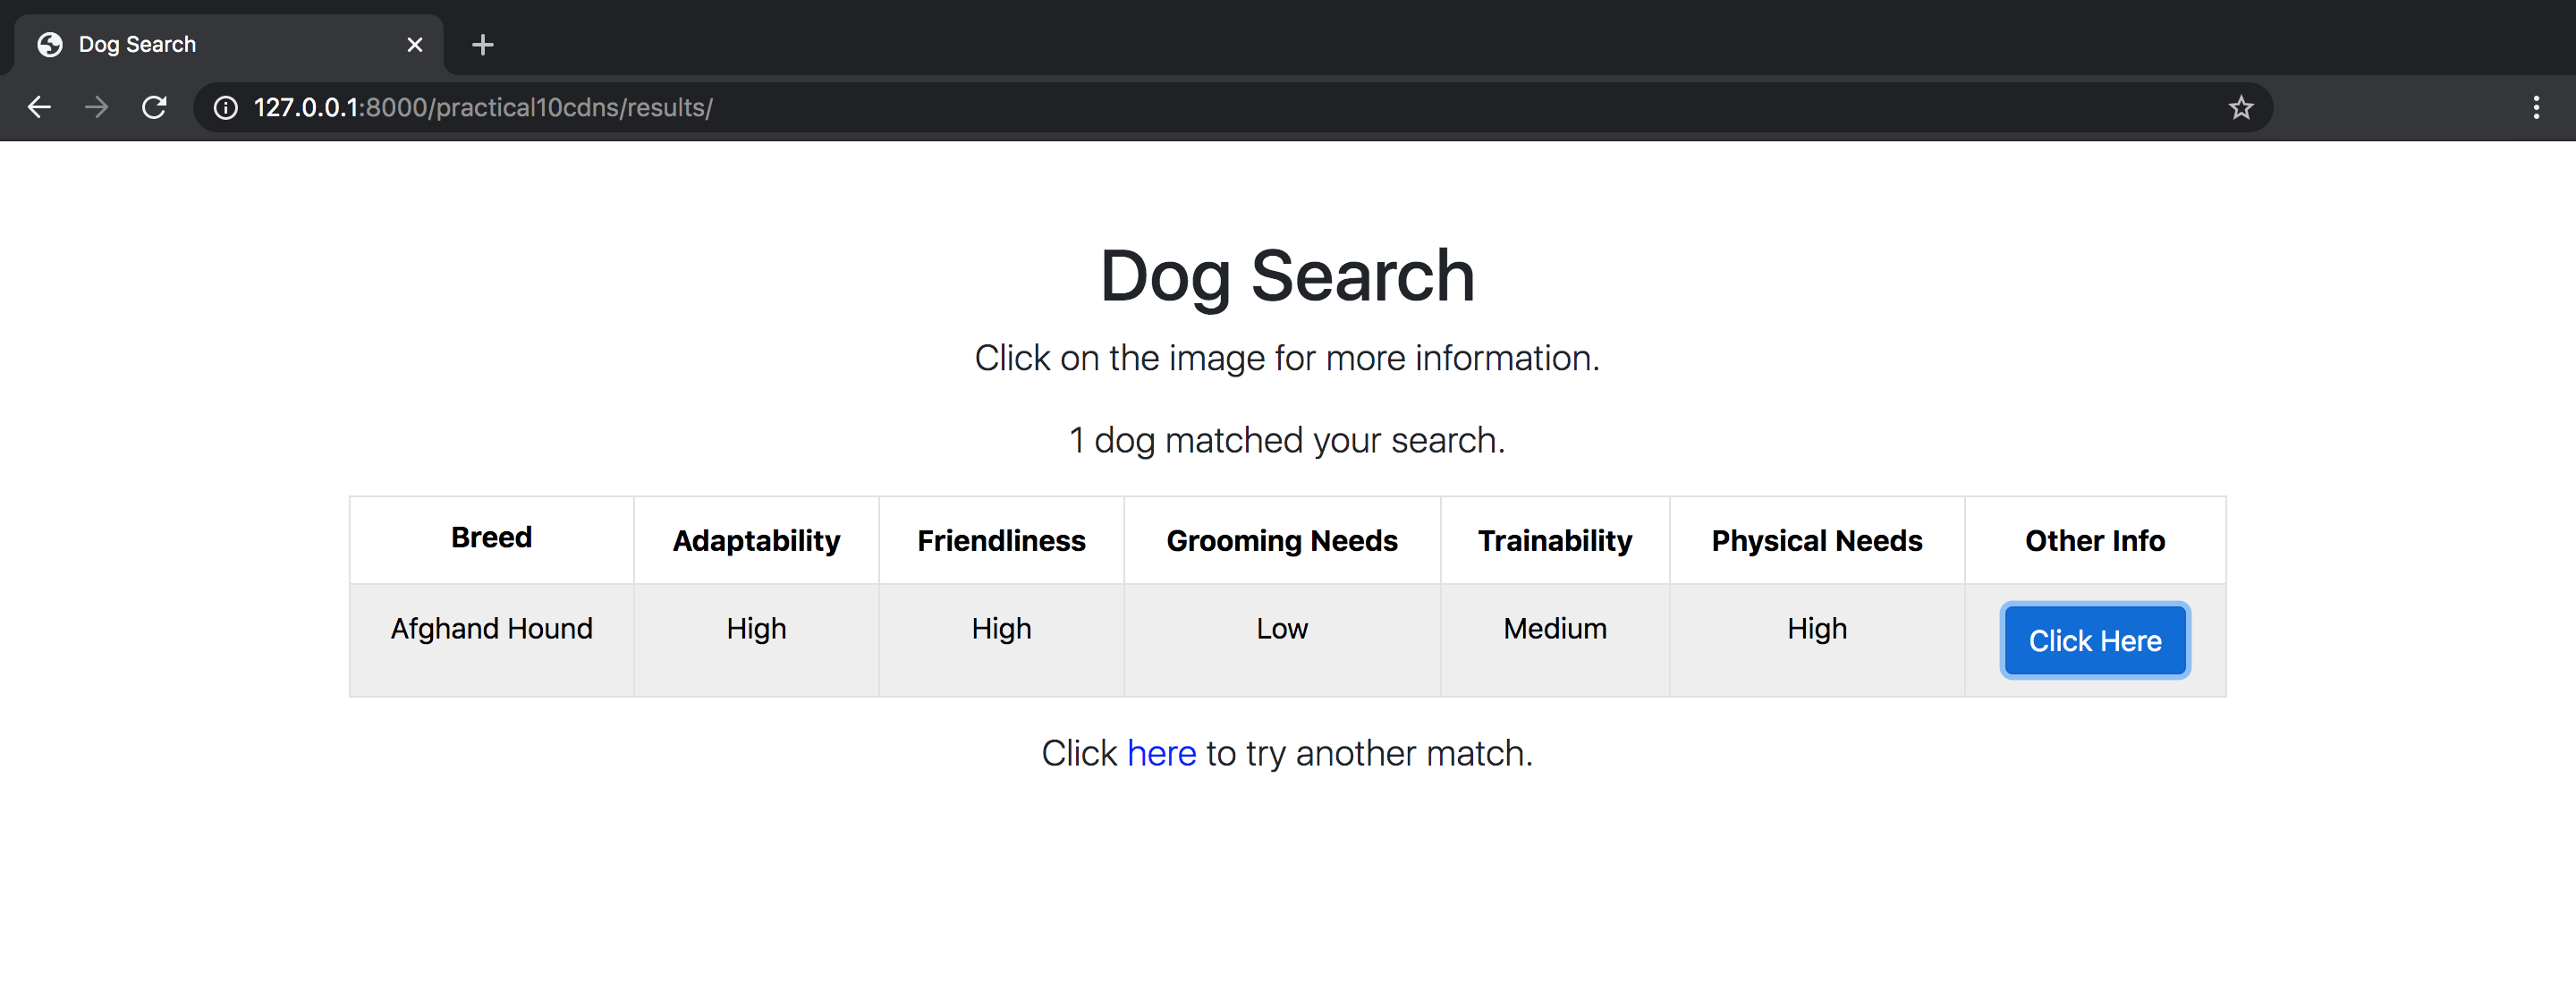
\includegraphics[width=175mm, height=65mm]{./img/10-expected-dog-search-6.png}
  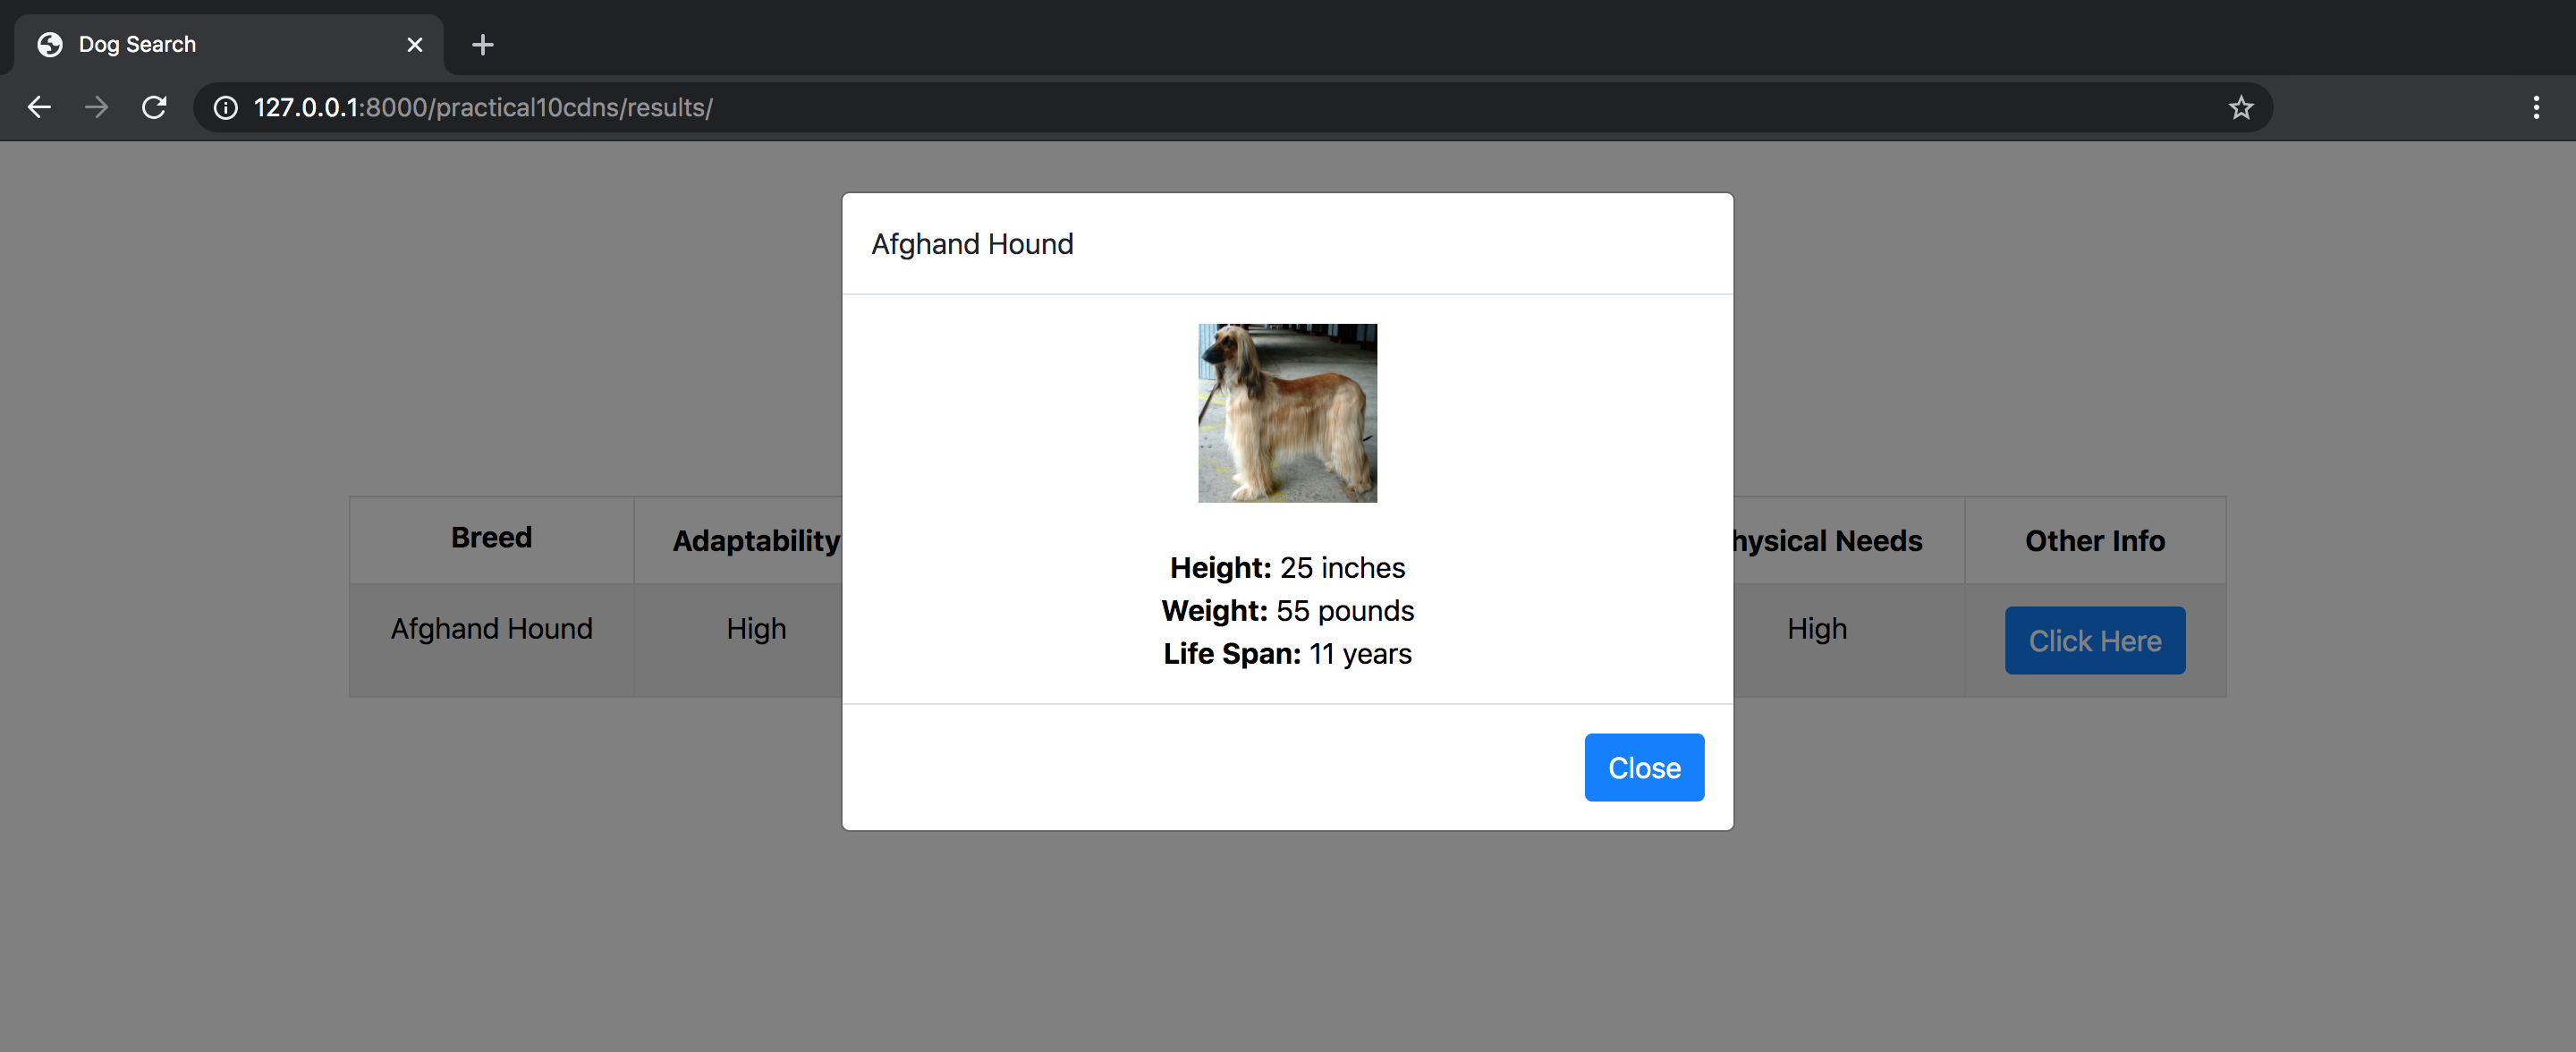
\includegraphics[width=175mm, height=65mm]{./img/10-expected-dog-search-7.png}
\end{figure}

\textbf{Deployment link:} \href{https://int-app-dev-practical-10.herokuapp.com/practical10cdns/}{https://int-app-dev-practical-10.herokuapp.com/practical10cdns/}

\subsection*{Resources} 
\begin{itemize}
  \item \href{https://pillow.readthedocs.io/en/3.0.x/index.html}{Pillow}
  \item \href{https://getbootstrap.com/}{Bootstrap}
\end{itemize}

\end{document}